\chapter{Introduction}

Infectious diseases have played an undeniably important role in human history. With human populations becoming sufficiently aggregated to sustain direct life cycle viral and bacterial infectants around 2000 BC, devastating invasions of a growing number of pathogens started to occur \citep{Dobson1996}.

One of the earliest well documented incidence of a large-scale epidemic is known as the Plague of Athens. Starting in 430 BC and lasting roughly three years, a highly infectious disease killed 75'000 to 100'000 people or 25\% of Athen's population. This catastrophic event is attributed either to smallpox, a viral infection with \textit{Variola major} of typhus, caused by \textit{Rickettsia} bacteria \citep{Littman2009}.

The bacterium \textit{Yersinia pestis} is responsible for three major plague pandemics in the early and late middle ages, as well as in the late 19th century. Originating in northern Africa in 523 AD and spreading around the Mediterranean basin throughout the years 541--546, the Plague of Justinian is assumed to have killed up to half of the population of affected areas. The effect on cities was disproportionately severe. In Constantinople, for example, an estimated 230'000 people out of 375'000 lost their lives to the disease \citep{Treadgold1997}. Returning in the years 1347--1351, known today as the Black Death, a plague pandemic again wiped out around half of Europe's population. Death toll estimates range from 15 to 23.5 million \citep{Zietz2004}. Leaving behind a grim cultural heritage, this catastrophe had a lasting effect on economic and social structures in Europe. The third large-scale outbreak started around 1855 in southern China and quickly spread to Japan, Taiwan and India again wreaking havoc on the affected population.

Bringing diseases such as smallpox, measles (an infection with the Measles virus) and typhus to the Americas during the European invasion of the New World had grave repercussions for the indigenous population, carrying no natural resistance towards the newly introduced pathogens. It is estimated that the population of present-day Mexico fell from 20 million to 1.6 million over the course of the 16th century due to multiple disease epidemics, critically contributing to the successful colonization of the new continents \citep{Dobson1996}.

Cholera and influenza are further contagious diseases with high mortality rates, responsible for global epidemics. \textit{Vibrio cholerae}, a bacterium which infects the intestine, became widespread in the early 19th century and led to seven pandemics since, the last of which only started in 1961. Antibacterial treatment of sewage and purification of drinking water greatly help to prevent and contain spreading of the disease but in areas with inadequate sanitation, such as Haiti after the 2010 earthquake, it remains a pathogen difficult to control. The influenza virus causes seasonal epidemics characterized by low lethality rates among people with intact immune systems\footnote{In spite of low lethality, these seasonal epidemics still incur significant economic damages. The \cite{WHO2003} estimates annual health care costs and loss of productivity due to influenza at US \$71--176 billion for the United States of America alone.}. Irregularly occurring influenza pandemics, initiated by zoonosis of new virus strains, against which no natural immunity exists, however, are accompanied by much higher lethality rates. The most significant such event is known today as the Spanish flu pandemic of 1918, costing the lives of 50--100 million, nearly half of which were young, healthy adults \citep{Taubenberger2006}.

In addition to diseases plaguing humanity for centuries, new ones continually emerge. \Gls{hiv} is believed to have transferred from non-human primates in the early 20th century and the recent outbreaks of \gls{sars} and swine flu serve as reminders of such occurrences.



\begin{knitrout}
\definecolor{shadecolor}{rgb}{0.969, 0.969, 0.969}\color{fgcolor}\begin{figure}
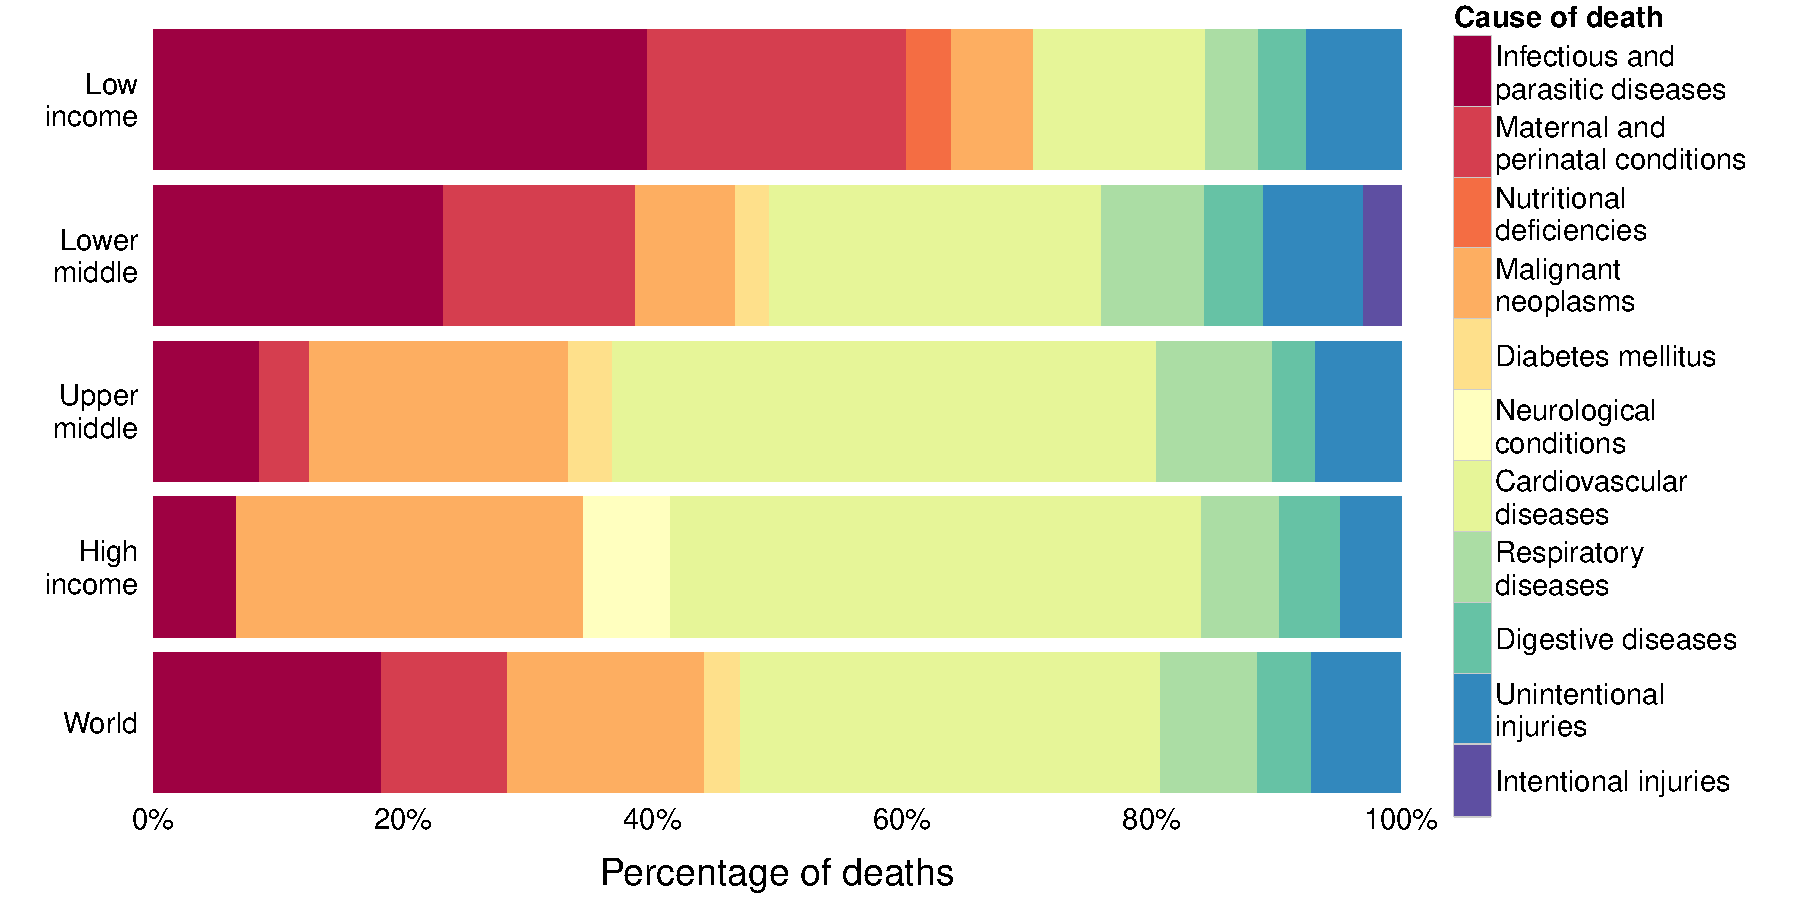
\includegraphics[width=\maxwidth]{figures/R/who-deaths/topCauses-who-deaths_top-causes-1} \caption[Relative frequencies of death causes in 2012 by World Bank income groups]{Relative frequencies of death causes in 2012 by World Bank income groups. Binning is based on Gross National Income (GNI) per capita and the thresholds are \$1'045 or less for low income, \$1046 to \$4125 for lower-middle, \$4126 to \$12745 for upper-middle and \$12746 or more for high income economies. The data was obtained from the \cite{WHO2012}.}\label{fig:who-deaths_top-causes}
\end{figure}


\end{knitrout}

\newcommand{\knitrTotalDeathsTwelve}{58.3 million}

\newcommand{\knitrPercentageDeathsTwelveHigh}{20.1\%}
\newcommand{\knitrPercentageDeathsTwelveLow}{14\%}
\newcommand{\knitrPercentageDeathsTwelveLmid}{36.5\%}
\newcommand{\knitrPercentageDeathsTwelveUmid}{29.4\%}

\newcommand{\knitrPercentDeathsTwelveLowInfect}{39.6\%}
\newcommand{\knitrPercentDeathsTwelveLowPerinat}{20.8\%}
\newcommand{\knitrPercentDeathsTwelveLmidInfect}{23.3\%}
\newcommand{\knitrPercentDeathsTwelveLmidCardio}{26.5\%}
\newcommand{\knitrPercentDeathsTwelveUmidInfect}{8.5\%}
\newcommand{\knitrPercentDeathsTwelveHighInfect}{6.7\%}
\newcommand{\knitrPercentDeathsTwelveWorldInfect}{18.3\%}
\newcommand{\knitrPercentDeathsTwelveWorldCardio}{33.7\%}


Despite development of means to treat and prevent many previously devastating diseases, infectious pathogens remain a serious threat to global health. In 2012, an estimated total of \knitrTotalDeathsTwelve{} people died (\knitrPercentageDeathsTwelveHigh{} in high, \knitrPercentageDeathsTwelveUmid{} in upper-middle, \knitrPercentageDeathsTwelveLmid{} in lower-middle and \knitrPercentageDeathsTwelveLow{} in low income countries). Figure \ref{fig:who-deaths_top-causes} partitions the total death count into World Bank income groups and causes. In low income countries, infective diseases are the most prevalent cause of death (\knitrPercentDeathsTwelveLowInfect{}), followed by maternal and perinatal complications with substantial margin (\knitrPercentDeathsTwelveLowPerinat{}). In lower middle income countries, cardiovascular conditions catch up (\knitrPercentDeathsTwelveLmidCardio{}), but are still almost matched in frequency by infectious diseases (\knitrPercentDeathsTwelveLmidInfect{}). In upper middle (\knitrPercentDeathsTwelveUmidInfect{}) and high income countries (\knitrPercentDeathsTwelveHighInfect{}), the importance of infectious disease while weakened remains accountable for a significant number of deaths. Globally, infectious diseases are the second most frequent cause of death (\knitrPercentDeathsTwelveWorldInfect{}), even more prevalent than all forms of cancer combined (\knitrPercentDeathsTwelveWorldCancer{}) and only preceded by cardiovascular diseases (\knitrPercentDeathsTwelveWorldCardio{}).

\begin{knitrout}
\definecolor{shadecolor}{rgb}{0.969, 0.969, 0.969}\color{fgcolor}\begin{figure}
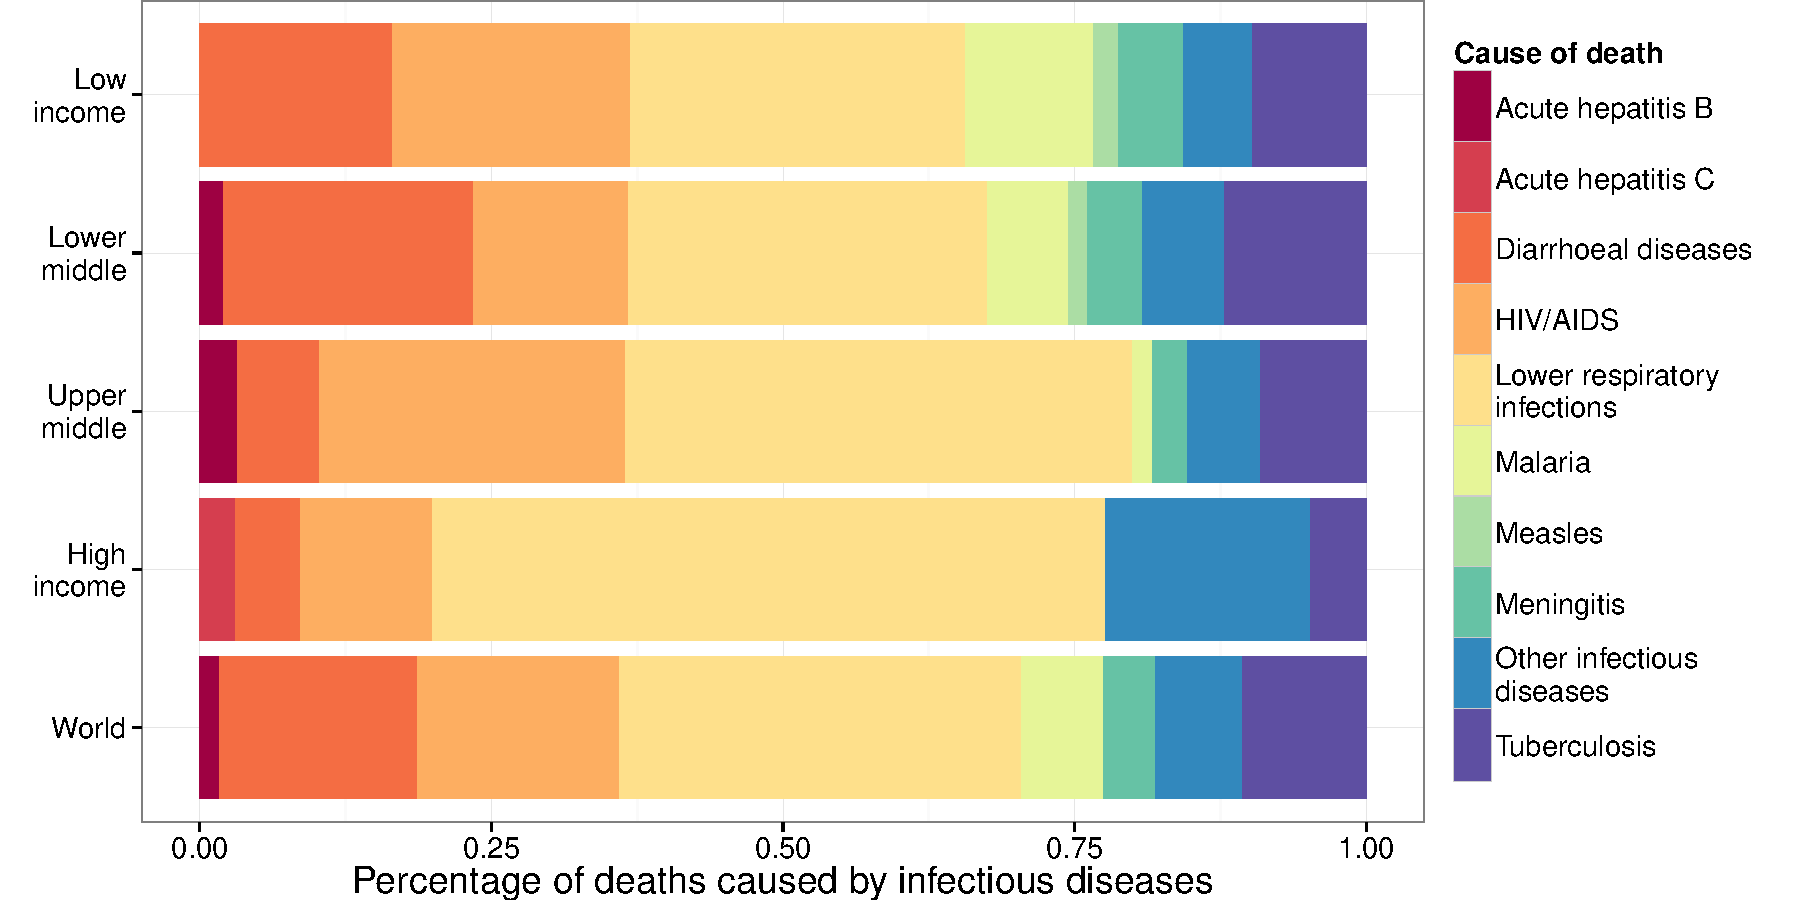
\includegraphics[width=\maxwidth]{figures/R/who-deaths/byDisease-who-deaths_by-disease-1} \caption[Relative frequencies deadly infectious diseases for 2012 by World Bank income groups]{Relative frequencies of deadly infectious diseases for 2012 by World Bank income groups. Binning is based on Gross National Income (GNI; see figure \ref{fig:who-deaths_top-causes}). The data was obtained from the \cite{WHO2012}.}\label{fig:who-deaths_by-disease}
\end{figure}


\end{knitrout}

\newcommand{\knitrPercentageInfectTwelveWorldLRI}{34.5\%}
\newcommand{\knitrPercentageInfectTwelveHighLRI}{57.7\%}
\newcommand{\knitrPercentageInfectTwelveUmidLRI}{43.5\%}
\newcommand{\knitrPercentageInfectTwelveLmidLRI}{30.8\%}
\newcommand{\knitrPercentageInfectTwelveLowLRI}{28.7\%}
\newcommand{\knitrPercentageInfectTwelveHighDiarr}{5.6\%}
\newcommand{\knitrPercentageInfectTwelveUmidDiarr}{7\%}
\newcommand{\knitrPercentageInfectTwelveLmidDiarr}{21.4\%}
\newcommand{\knitrPercentageInfectTwelveLowDiarr}{16.6\%}
\newcommand{\knitrPercentageInfectTwelveWorldAIDS}{17.3\%}
\newcommand{\knitrPercentageInfectTwelveWorldDiarr}{16.9\%}
\newcommand{\knitrPercentageInfectTwelveHighAIDS}{11.3\%}
\newcommand{\knitrPercentageInfectTwelveUmidAIDS}{26.2\%}
\newcommand{\knitrPercentageInfectTwelveLmidAIDS}{13.3\%}
\newcommand{\knitrPercentageInfectTwelveLowAIDS}{20.4\%}


Focusing only on deaths caused by infectious disease, lower respiratory infections are most frequent (for each income region individually, low to high: \knitrPercentageInfectTwelveLowLRI{}, \knitrPercentageInfectTwelveLmidLRI{}, \knitrPercentageInfectTwelveUmidLRI{} and \knitrPercentageInfectTwelveHighLRI{} as well as worldwide: \knitrPercentageInfectTwelveWorldLRI{}; cf. figure \ref{fig:who-deaths_by-disease}). Diarrhoeal diseases and HIV\slash AIDS are the next most common worldwide (\knitrPercentageInfectTwelveWorldDiarr{} and \knitrPercentageInfectTwelveWorldAIDS{}, respectively) where diarrhea is more prevalent in lower income regions (\knitrPercentageInfectTwelveLowDiarr{} and \knitrPercentageInfectTwelveLmidDiarr{} versus \knitrPercentageInfectTwelveUmidDiarr{} and \knitrPercentageInfectTwelveHighDiarr{}), while HIV\slash AIDS plays a major role irrespective of income region (low to high: \knitrPercentageInfectTwelveLowAIDS{}, \knitrPercentageInfectTwelveLmidAIDS{}, \knitrPercentageInfectTwelveUmidAIDS{} and \knitrPercentageInfectTwelveHighAIDS{}).

Dealing with highly virulent pathogens and preventing their spreading requires a multi-pronged approach. First and foremost, etiology and routes of transmission have to be understood. Knowledge of vectors and natural reservoirs is of great importance as a first line of defense. In the case of plague, for example, insecticides killing fleas were successfully used as a prophylactic measure, as was controlling rat populations \citep{Barnes1990}. Sanitary precautions including purification of drinking water, cocking foods well and the usage of disinfectants prevent initial infection, while measures such as sewage treatment, hand washing and wearing face masks help limiting spread among humans. Vaccination is the most important preventive measure. Exposing the immune system to a foreign antigen in a controlled manner artificially induces immunity. Among the great successes of widespread vaccination efforts is the global eradication of smallpox through a coordinated initiative lead by the World Health Organization in the 1970's.

Post-infection therapies include symptomatic treatments, as well as anti-in\-fec\-tive drugs. Anti-bacterial or anti-viral agents exploit differences in proteomes between host and pathogen to selectively disable the invader with minimal toxicity to the host. This approach has been tremendously successful throughout most of the 20th century, leading to widespread application and prompting development of resistance towards the commonly used compounds. Adding to the severity of the problem is a lack of discovery of new drugs. No new class of anti-bacterial agents has been found since 1987, causing big pharmaceutical companies to withdraw from the area. The remaining research is mainly focused on improving on existing drugs, leading to a weak product pipeline, especially for the treatment of gram-negative bacteria \citep{Silver2011}. In its first global study on anti-microbial resistance, the \cite{WHO2014} notes:

\begin{quote}
\Gls{amr} within a wide range of infectious agents is a growing public health threat of broad concern \ldots A post-antibiotic era—-in which common infections and minor injuries can kill—-far from being an apocalyptic fantasy, is instead a very real possibility for the 21st century.
\end{quote}

An alternative to pathogen directed search lies in targeting the set of host proteins necessary for infection. Many intracellular parasites subvert cellular functions to gain entry via host-mediated processes such as endocytosis. Upon entry, they move to a suitable niche and rely on host resources for proliferation. Challenges include evading host-cell defense mechanisms, generating sufficient space for replication, nutrient acquisition and keeping the host alive as long as possible, most of which require complex interactions between invader and host-based mechanisms. Finally, exiting the host cell again requires the parasite to successfully insert itself into existing signaling pathways \citep{Leiriao2004}.

\Gls{hdt} offer an escape from the conundrum of wanting to combat but not wanting to select for the surviving microbial parasites. The major challenge under this regimen is finding infectome components that are nonessential for cell survival, as orthogonality of host and infectant can no longer be exploited. Proving feasibility of the approach, \citeauthor{Czyz2014} screened a library of 640 compounds already approved by the United Stated Food and Drug Administration (USFDA or short FDA) for inducing resistance to four intracellular pathogens (\textit{Coxiella burnetii}, \textit{Legionella pneumophila}, \textit{Brucella abortus}, and \textit{Rickettsia conorii}). They found multiple drugs, not classified as antibiotics, that successfully inhibited intracellular bacterial growth while entailing only limited toxicity to THP-1 host cells. \citeauthor{Prussia2011} review the usage of genome-wide screens to study host-pathogen interactions (for HIV and influenza) which in turn serve as basis for rational identification of drug targets for novel host-directed antivirals. \nocite{Hawn2015}

A detailed understanding of the human infectome is of crucial importance to the development of \gls{hdt} and may even benefit the development of new anti-microbial agents. Feasibility of systematic loss of function screens using \gls{rna} interference methodology offers a unique opportunity to investigate complex cellular networks, making this an ideal tool for laying groundwork in combating infectious diseases. Of great importance, however, is ensuring reproducibility and comparability of such datasets, as well as ready availability to the scientific community.

Created to tackle such issues, InfectX and TargetInfectX are two successive \gls{rtd} projects funded by SystemsX, the Swiss initiative for systems biology, contracted with identification and study of the human infectome for a set of bacterial (\textit{Bartonella henselae}, \textit{Brucella abortus}, \textit{Listeria monocytogenes}, \textit{Salmonella} typhimurium and \textit{Shigella flexneri}) and viral pathogens (adenovirus, rhinovirus and \textit{Vaccinia virus}). The central effort of generating kinome- and genome-wide \gls{sirna} screens for each of the investigated pathogens and capturing image data followed by computational image analysis is carried out by an interdisciplinary consortium of research groups spanning the Universities of Basel and Z\"urich, the Swiss Federal institute of Technology (ETH Z\"urich), as well as the Pasteur Institute.

A wealth of data is easily generated by running computational feature recognition at single cell resolution on microscopic images which subsequently calls for sophisticated statistical analysis in order to expose biologically relevant information. This master thesis explores the single cell feature space, provides software to handle such datasets and attempts to employ \glspl{glm} for comparing \gls{sirna}-knockdown experiments and identifying discriminatory features. Following this introductory part, chapter 2 will provide the necessary biological background, covering microbial infection mechanisms, a description of each pathogen in terms of physical characteristics, diseases caused, pathogenesis and epidemiology, as well as giving an introduction on \gls{rna} interference, including molecular mechanism, biological function and several applications alongside methodological caveats. Chapter 3 reviews InfectX data collection, detailing experimental setup, image acquisition, data processing and image analysis, as well as qualitatively describing the available datasets.

An R package called singleCellFeatures was developed to facilitate working with single cell feature datasets, the specifics of which are detailed in chapter 4. Beginning with a motivational example, the importance of efficient computation and data representation is highlighted and the R package is described in terms of developed S3 classes as well as data fetching, caching, manipulation and analysis routines. Finally, chapter 5 introduces \glspl{glm}, \glspl{pmm}, deliberates several normalization approaches and concludes with some analysis results along with a discussion of unresolved issues.

